
%%% \FloatBarrier
\section{Map-based Skeletons}
\label{sec:map-skeletons}
Now we have developed Parallel Arrows far enough to define some useful algorithmic skeletons that abstract typical parallel tasks.

\subsection{Parallel map}

\begin{figure}[h]
%parMap
\includegraphics[scale=0.7]{images/parMap}
\caption{Schematic depiction of |parMap|.}
\label{fig:parMapImg}

\begin{code}
parMap :: (ArrowParallel arr a b conf) => conf -> (arr a b) -> (arr [a] [b])
parMap conf f = parEvalN conf (repeat f)
\end{code}
\caption{Definition of parMap.}
\label{fig:parMap}

%parMapStream
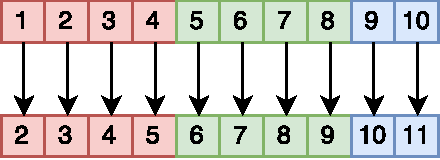
\includegraphics[scale=0.7]{images/parMapStream}
\caption{Schematic depiction of parMapStream.}
\label{fig:parMapStreamImg}

\begin{code}
parMapStream :: (ArrowParallel arr a b conf, ArrowChoice arr, ArrowApply arr) =>
	conf -> ChunkSize -> arr a b -> arr [a] [b]
parMapStream conf chunkSize f = parEvalNLazy conf chunkSize (repeat f)
\end{code}
\caption{Definition of |parMapStream|.}
\label{fig:parMapStream}
\end{figure}

The |parMap| skeleton (Figs.~\ref{fig:parMapImg},~\ref{fig:parMap}) is probably the most common skeleton for parallel programs. We can implement it with |ArrowParallel| by repeating an arrow |arr a b| and then passing it into |parEvalN| to get an arrow |arr [a] [b]|.
Just like |parEvalN|, |parMap| is 100\% strict.

\paragraph{Lazy parallel map}
As |parMap| (Figs.~\ref{fig:parMapImg},~\ref{fig:parMap}) is 100\% strict it has the same restrictions as |parEvalN| compared to |parEvalNLazy|. So it makes sense to also have a |parMapStream| (Fig.~\ref{fig:parMapStreamImg},~\ref{fig:parMapStream}) which behaves like |parMap|, but uses |parEvalNLazy| instead of |parEvalN|.

\subsection{Statically load-balancing parallel map}

\begin{figure}[h]
%farm
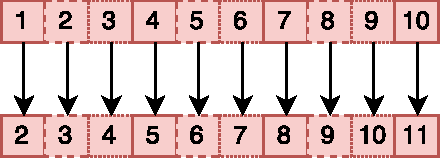
\includegraphics[scale=0.7]{images/farm}
\caption{Schematic depiction of a |farm|, a statically
      load-balanced |parMap|.}
\label{fig:farmImg}

\begin{code}
farm :: (ArrowParallel arr a b conf,
	ArrowParallel arr [a] [b] conf, ArrowChoice arr) =>
	conf -> NumCores -> arr a b -> arr [a] [b]
farm conf numCores f =
	unshuffle numCores >>>
	parEvalN conf (repeat (mapArr f)) >>>
	shuffle
\end{code}
\caption{The definition of |farm|.}
\label{fig:farm}

%farmChunk
\includegraphics[scale=0.7]{images/farmChunk}
\caption{Schematic depiction of farmChunk.}
\label{fig:farmChunkImg}
\end{figure}

A |parMap| (Figs.~\ref{fig:parMapImg},~\ref{fig:parMap}) spawns every single computation in a new thread (at least for the instances of |ArrowParallel| we gave in this paper). This can be quite wasteful and a |farm| (Fig.~\ref{fig:farmImg},~\ref{fig:farm}) that equally distributes the workload over |numCores| workers (if numCores is greater than the actual processor count, the fastest processor(s) to finish will get more tasks) seems useful.
The definitions of the helper functions |unshuffle|, |takeEach|, |shuffle| (Fig.~\ref{fig:edenshuffleetc}) originate from an Eden skeleton\footnote{Available on Hackage under \url{https://hackage.haskell.org/package/edenskel-2.1.0.0/docs/src/Control-Parallel-Eden-Map.html}.}.

\paragraph{Lazy statically load-balancing parallel map}
Since a |farm| (Fig.~\ref{fig:farmImg},~\ref{fig:farm}) is basically just |parMap| with a different work distribution, it is, again, 100\% strict. So we can define |farmChunk| (Fig.~\ref{fig:farmChunkImg},~\ref{fig:farmChunk}) which uses |parEvalNLazy| instead of |parEvalN|. It is basically the same definition as for |farm|, with |parEvalN| replaced with |parEvalNLazy|.

%%% Local Variables:
%%% mode: latex
%%% TeX-master: "main"
%%% End:
